\section{Kombinatorik}

\subsection{Zählregeln}

\begin{minipage}[t]{0.48\columnwidth}
	\begin{center}
		\myul{\textbf{Disjunkte Vereinigung}}

		\vspace{0.2cm}

		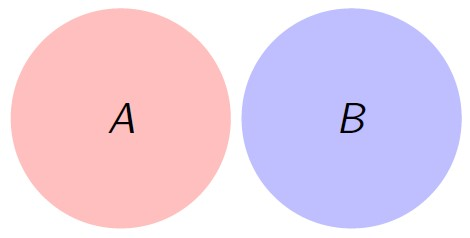
\includegraphics[height=2cm]{images/disjunkte_vereinigung.jpg}
		$$ \crd{A} \cup \cbl{B} | = | \crd{A} | + | \cbl{B} | $$
	\end{center}
\end{minipage}
\hfill
\begin{minipage}[t]{0.48\columnwidth}
	\begin{center}
		\myul{\textbf{Schnittmengen}}

		\vspace{0.2cm}

		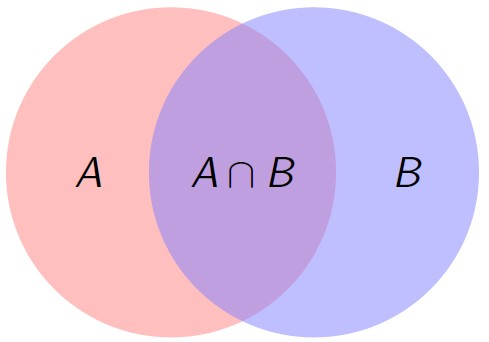
\includegraphics[height=2cm]{images/schnittmenge.jpg}
		$$ | \crd{A} \cup \cbl{B} | = | \crd{A} | + | \cbl{B} | - | \crd{A} \cap \cbl{B} | $$
	\end{center}
\end{minipage}

\vspace{0.2cm}
$$ | A \cup B \cup C | = |A| + |B| + |C| - |A \cap B| - |A \cap C| - |B \cap C| + |A \cap B \cap C| $$


\vspace{0.1cm}


\begin{minipage}[t]{0.48\columnwidth}
	\begin{center}
		\myul{\textbf{Paare = Produkt}}

		\vspace{0.2cm}

		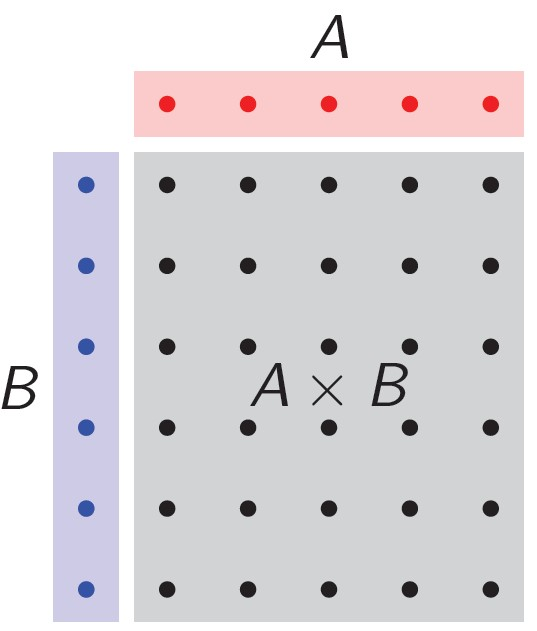
\includegraphics[width=0.7\columnwidth]{images/paare_produkt.jpg}
		$$ | \crd{A} \times \cbl{B} | = | \crd{A} | \cdot | \cbl{B} | $$	
	\end{center}
\end{minipage}
\hfill
\begin{minipage}[t]{0.48\columnwidth}
	\begin{center}
		\myul{\textbf{Produktregel}}
	\end{center}

	Für-jeden-gibt-es-Regel

	\vspace{0.2cm}

	\crd{Wichtigste Regel in der Kombinatorik} 

	\vspace{0.2cm}

	Wenn es für jede von $n$ Wahl-möglichkeiten $m$ mögliche weitere Wahlmöglichkeiten gibt, 
	dann gibt es insgesamt $n \cdot m$ Möglichkeiten 
\end{minipage}


\subsection{Anordnungsproblem / Reihefolge (Permutation)}

\textbf{Auf wie viele Arten kann man $\bm{n}$ Objekte (auf $\bm{n}$ Plätzen) anordnen?} \\
\textrightarrow\ Reihenfolge relevant, keine Wiederholungen
$$ \boxed{ \text{\#} \; \text{Möglichkeiten} = P_n = n! }$$


\subsection{Perlenkette (Variation)}
\textbf{Auf wie viele Arten kann man $\bm{k}$ mal unter $\bm{n}$ verschiedenen Objekte auswählen?}

\vspace{0.1cm}
\textbf{Auf wieviele Arten kann man eine Perlenkette der Länge $\bm{k}$ aus $\bm{n}$ Farben von Perlen herstellen?} \\
\textrightarrow\ Reihenfolge egal, Wiederholungen erlaubt; 'Ziehen mit zurücklegen'
$$\boxed{ \text{\#} \; \text{Möglichkeiten} = V_{n,k} = n^k } $$ 


\subsection{Auswahlproblem (Kombination)}

\textbf{Auf wieviele Arten kann man $\bm{k}$ Objekte aus $\bm{n}$ auswählen? (Lottoproblem)} \\
\textrightarrow\ Reihenfolge egal, keine Wiederholungen; 'Ziehen ohne zurücklegen'

$$\boxed{ \text{\#} \; \text{Möglichkeiten} = C_k^n = \frac{n!}{k! \, (n-k)!} = 
\begin{pmatrix} n \\ k \end{pmatrix} } $$ 

Taschenrechner: nCr($n, \, k$)


\subsection{Tipps und Tricks zu Kombinatorik}
\begin{itemize}
	\item Aufgabe in oben beschriebene Teilprobleme aufteilen
	\item Teillösungen \textbf{multiplizieren}
\end{itemize}


\subsection{Erzeugende Funktion}

Für $a_k \in \mathbb{R}, \; k = 0, \, 1, \, ...$, heisst $f(z)$ die \textbf{erzeugende Funktion} der Koeffizienten $a_k$
$$ f(z) = \sum\limits_{k=0}^\infty a_k \, z^k $$

\textrightarrow\ Die Funktion $f(z)$ erzeugt die Koeffizienten $a_k$ eines Polynoms der Form
$$ a_0 \, z^0 + a_1 \, z^1 + a_2 \, z^2 + ... + a_k \, z^k $$ 


\subsubsection{Beispiele für erzeugende Funktionen}

\begin{itemize}
	\setlength\itemsep{0.75em}
	\item $f(z) = \cbl{1} + \cor{1} \, z$ ist erzeugende Funktion von $a_k = (\cbl{1}, \, \cor{1}, \,0, \,0, \, ...)$
	\item $a_k = (\cbl{1}, \, \cor{2}, \, \cgn{3}, \, \crd{4})$ \textrightarrow\  $f(z) = \cbl{1} + \cor{2} \, z + \cgn{3} \, z^2 + \crd{4} \, z^3$
	\item $f(z) = (1 + z)^n$ ist erzeugende Funktion der Binomialkoeffizienten $a_k = \begin{pmatrix} n\\k \end{pmatrix}$
\end{itemize}


\vfill\null
\columnbreak


\subsubsection*{Anwendung: Münzwechsel}

\textbf{Gegeben:} 3 Einfränkler, 4 Zweifränkler, 7 Fünfliber \\
\textbf{Gesucht:} Auf wieviele Arten kann man jeden möglichen Betrag $k$ damit zahlen?

\vspace{0.2cm}

\begin{tabular}{ll}
	$0-3$ Einfränkler:	& $f_1(z) = 1 + z^1 + z^2 + z^3$ \\	
	$0-4$ Zweifränkler: & $f_2(z) = 1 + \cbl{0} \, z^{\cor{1}} + \cbl{1} \, z^{\cor{2}} + \cbl{0} \, z^{\cor{3}} + \cbl{1} z^{\cor{4}} + \ldots + \cbl{1} \, z^{\cor{8}}$ \\	
	$0-7$ Fünfliber: 	& $f_5(z) =  1 + 1 \, z^5 + 1 \, z^{10} + \ldots + 1 \, z^{35} $ \\	
	Alle Werte: 		& $f_1(z) \cdot f_2(z) \cdot f_5(z)$
\end{tabular}

\vspace{0.2cm}

\textrightarrow\ $\text{\cbl{{\# Mögl. um Betrag zu erreichen}}} \; z^{\cor{\text{Betrag in CHF}} }$

\vspace{0.3cm}

\textbf{\myul{Wichtige Erkenntnis zur formalen Variable \(z\):}}
\begin{itemize}
	\setlength\itemsep{0.5em}
	\item \(z\) ist lediglich ein \textbf{formaler Platzhalter}. Es wird \textbf{kein konkreter Wert} für \(z\) eingesetzt!
	\item Der \textbf{Exponent} von \(z\) entspricht dem \textbf{Geldbetrag} (in CHF).
	\item Der \textbf{Koeffizient} vor dem \(z\) entspricht der \textbf{Anzahl der Möglichkeiten}, diesen Betrag zu erreichen.
\end{itemize}

\vspace{0.2cm}

\textbf{Vorgehen beim Auswerten:}
\begin{enumerate}
	\setlength\itemsep{0.5em}
	\item Multipliziere die erzeugenden Funktionen \(f_1(z) \cdot f_2(z) \cdot f_5(z)\) vollständig aus.
	\item Durch die Polynommultiplikation addieren sich die Exponenten (\(z^a \cdot z^b = z^{a+b}\)). Das entspricht genau dem Addieren der Geldwerte der kombinierten Münzen.
	\item Suche im ausmultiplizierten Polynom den Term mit dem gewünschten Exponenten \(z^k\) (z.B. \(z^5\) für genau 5 CHF).
	\item Die Zahl vor diesem Term (der Koeffizient) ist die gesuchte Anzahl an Kombinationsmöglichkeiten.
\end{enumerate}

\vspace{0.2cm}
\textit{Beispiel:} Der Koeffizient von \(z^5\) im Endergebnis gibt an, auf wie viele Arten man genau 5 CHF mit den gegebenen Münzen bezahlen kann.

